\section{Durchführung}
\label{sec:Durchführung}

Zur Durchführung des Versuches stehen ein Ultraschallechoskop, zwei $2 \unit{\mega\hertz}$-Ultraschallsonden sowie ein Computer zur Datenaufnahme und -analyse bereit.
Das Echoskop kann dabei mithilfe eines Reglers auf das Impuls-Echo-Verfahren bzw. das Durchschallungsverfahren eingestellt werden. \\

Die zu untersuchenden Acrylproben werden dabei je nach Lage mit bidestilliertem Wasser bzw. Kopplungsgel gekoppelt, um den bestmöglichen Kontakt zu ermöglichen. \\


\subsection{Vorbereitung}

Um sich mit dem Gerät sowie \textit{EchoView}, dem zur Messdatenverarbeitung verwendeten Programm, vertraut zu machen, soll zunächst eine Längenbestimmung über die Schallgeschwindigkeit in Acryl durchgeführt werden.
Die Dicker einer der Acrylplatten wird mithilfe der Schieblehre vermessen. Anschließend wird die Sonde von oben mit destilliertem Wasser gekoppelt. %Korrektur
Über die Verzögerung zwischen zwei Impulsen lässt sich die Schallgeschwindigkeit bestimmen, mithilfe derer eine Längenmessung durchgeführt werden kann. \\


\subsection{Schallgeschwindigkeitsbestimmung über das Impuls-Echo-Verfahren}

Nun soll die Schallgeschwindigkeit in Acryl mithilfe des Impuls-Echo-Verfahrens bestimmt werden.
Dazu werden, analog zur bereits beschriebenen Messung, mithilfe der Schieblehre die Dicken der gestellten Acrylzylinder ermittelt.
Die Zylinder werden daraufhin mit destilliertem Wasser an die Ultraschallsonde gekoppelt. Aus der Verzögerung zwischen Ausgangsimpuls und Eingangsimpuls wird die Schallgeschwindigkeit bestimmt. %Korrektur
Diese Messung wird für insgesamt sieben Längen durchgeführt, wobei einige Längen durch Kopplung kürzerer Einzelzylinder zusammengesetzt werden. \\


\subsection{Schallgeschwindigkeitsbestimmung über das Durchschallungsverfahren}

Dieselbe Messung wird anschließend mithilfe des Durchschallungsverfahrens wiederholt.
Dazu werden die Zylinder horizontal auf eine Halterung gelegt. An beiden Enden wird mit Kopplungsgel eine der beiden Sonden gekoppelt. %Korrektur
Aus der Durchlaufzeit wird die Schallgeschwindigkeit bestimmt und anschließend mit dem Impuls-Echo-Verfahren verglichen. \\


\subsection{Dämpfungsbestimmung über das Impuls-Echo-Verfahren}

Die zu untersuchenden Zylinder werden erneut aufrecht gestellt und von oben mit einer Sonde gekoppelt.
Es wird die Amplitudendifferenz zwischen dem ausgesendeten und reflektierten Impuls gemessen, wobei der Verstärkungsfaktor dringenst beachtet werden muss.%Korrektur
Die Messung wird für sechs Längen durchgeführt. Mithilfe der aufgenommenen Daten wird anschließend die Dämpfung bestimmt. %Korrektur


\subsection{Biometrische Untersuchung eines Augenmodells}

Anhand des in \autoref{fig:abb3} dargestellten Augenmodells sollen die Abmessungen des Auges aufgenommen werden.
Dazu werden die Laufzeiten an der Iris sowie der Retina aufgenommen, mithilfe der Schallgeschwindigkeiten in der Linse und der Glaskörperflüssigkeit werden die Abmessungen bestimmt.
\begin{figure}
    \centering
    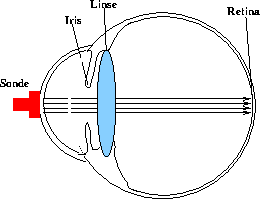
\includegraphics{figures/abb3.pdf} 
    \caption{Querschnitt des Augenmodells\cite{ap06}.}
    \label{fig:abb3}
\end{figure}






